\PassOptionsToPackage{unicode}{hyperref}
\documentclass[aspectratio=1610, 9pt]{beamer}

% Load packages you need here
\usepackage{polyglossia}
\setmainlanguage{german}

\usepackage{csquotes}
\usepackage{graphicx}
\usepackage{siunitx}
\usepackage{amsmath}
\usepackage{amssymb}
\usepackage{mathtools}

\usepackage{hyperref}
\usepackage{bookmark}

% load the theme after all packages

\usetheme[
  showtotalframes, % show total number of frames in the footline
   dark, % optional dark theme, uncomment to use
]{tudo}

% Put settings here, like
\unimathsetup{
  math-style=ISO,
  bold-style=ISO,
  nabla=upright,
  partial=upright,
  mathrm=sym,
}
\begin{document}
\title{Observing the Prompt Component of the Atmospheric Muon Flux Using IceCube}
\author{Leander Flottau}
%\institute{Astroteilchenphysik \\  Fakultät: Physik}
\titlegraphic{
\includegraphics[width=0.7\textwidth]{Plots/IceCube_webheader_fullcolor}}
\begin{document}
\maketitle
%\begin{frame}
%  \frametitle{Table of Contents}
%  \tableofcontents
%\end{frame}  
%\section{IceCube Neutrino Observatory}
\begin{frame}
    \section{IceCube Neutrino Observatory}
    \begin{minipage}{0.6\textwidth}
        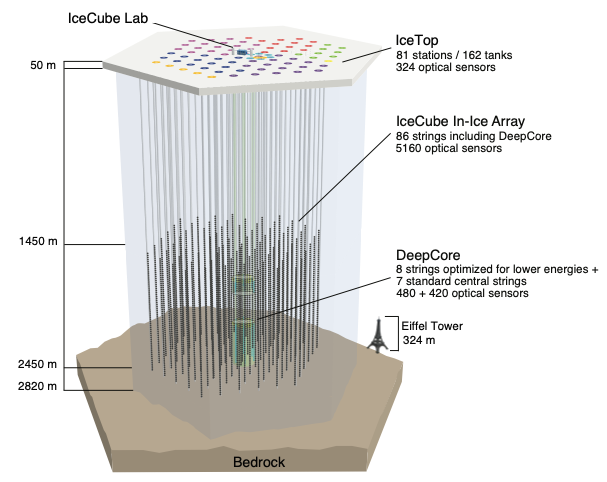
\includegraphics[width=\textwidth]{Plots/IceCube schematic}
    \end{minipage}
    \begin{minipage}{0.39\textwidth}
        \begin{itemize}
            \item Cubic kilometer scale cherenkov detector
            \item $5160$ DOMs on $86$ strings
            \item $\approx 270$ measured Nutrino Events per day
            \item $\approx \SI{3}{\kilo\hertz}$
        \end{itemize}
    \end{minipage}
\end{frame}
\begin{frame}
    \section{Atmospheric Air Showers}
    \begin{minipage}{0.6\textwidth}
        \includegraphics[width=\textwidth]{Plots/Air Shower Illustration}
    \end{minipage}
    \begin{minipage}{0.39\textwidth}
        \begin{itemize}
            \item Cosmic ray interactions produce secondary particles
            \item Major decay product: $\mu$
        \end{itemize}
    \end{minipage}
\end{frame}
\begin{frame}
    \section{The Prompt Component}
    \begin{minipage}{0.6\textwidth}
        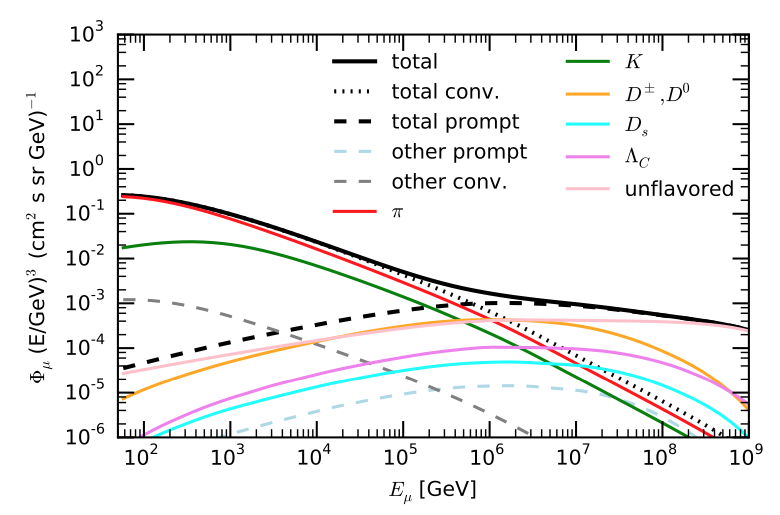
\includegraphics[width=\textwidth]{Plots/Prompt vs conventional flux}
    \end{minipage}
    \begin{minipage}{0.39\textwidth}
        \begin{itemize}
            \item Conventional: produced by $K^{\pm}$/$\pi^{\pm}$
            \item Prompt: produced by short lived particles
            \item Prompt dominant at high energies
        \end{itemize}
    \end{minipage}
\end{frame}
\begin{frame}
    \section{The Muon-Puzzle}
    \begin{minipage}{0.6\textwidth}
        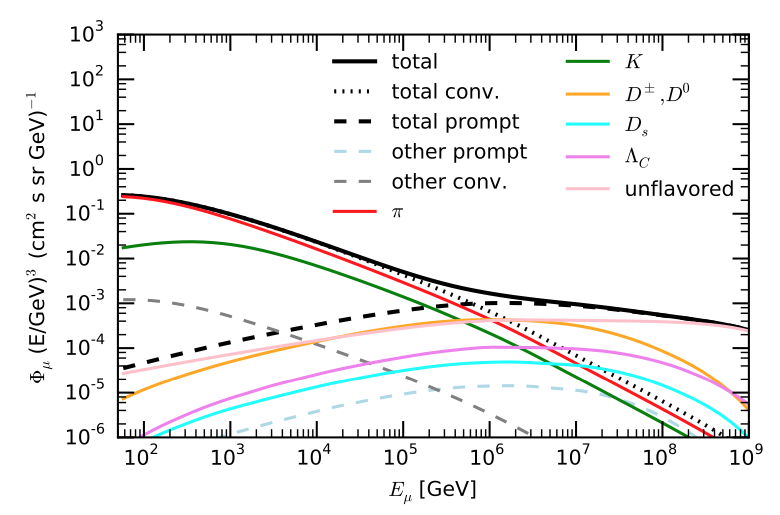
\includegraphics[width=\textwidth]{Plots/Prompt vs conventional flux}
    \end{minipage}
    \begin{minipage}{0.39\textwidth}
        \begin{itemize}
            \item More muons measured than simulations predicted
            \item Composition of secondary particles in cosmic ray interactions
            \item Hadronic interaction models
            \item Muons in IceCube: high energies and forward boosted
        \end{itemize}
    \end{minipage}
\end{frame}
\begin{frame}
    \frametitle{Simulations and tagging}
    \begin{itemize}
        \item Tagging of parent particles in CORSIKA simulations
        \item Prompt definition based on parent of leading muon
        \item Allows MC-Sample with prompt/conventional distinction 
    \end{itemize}
\end{frame}
\end{document}